\documentclass{article}
\usepackage{CJKutf8}
\usepackage{multicol}
% Packages
\usepackage{lipsum} % For generating dummy text
\usepackage[top=1in, bottom=1in, left=1in, right=1in]{geometry}
\usepackage{hyperref}
\usepackage{pgfplots}
\usetikzlibrary{pgfplots.polar}
\usepackage{caption}
\captionsetup{font=small}
\usepackage{standalone}
\usepackage{listings}
\usepackage{xcolor} % For setting colors
\usepackage{amssymb}
\usepackage{amsmath}
\usepackage{algorithm}
\usepackage{algpseudocode}
\usepackage{afterpage}
\usepackage{placeins}
\usepackage{tikz}
\usepackage{enumitem}
\lstset{
  language=[LaTeX]TeX,
  breaklines=true,
  basicstyle=\ttfamily\small,
  keywordstyle=\color{blue},
  commentstyle=\color{green},
  backgroundcolor=\color{gray!10},
  frame=single,
  showspaces=false,
  showstringspaces=false,
}
\pgfplotsset{compat=1.17} % Use this to ensure compatibility with newer features
\setlength{\parskip}{6pt}
% Title and author

\title{Autonomous Competence Identification Protocol: A Dynamic Ranking Ladder System for Blockchain Applications}

\author{Tim Pechersky, Aivars Smirnovs}

\begin{document}
\begin{CJK}{UTF8}{gbsn}

    % \twocolumn
    \maketitle

    \begin{abstract}
        Meritocratic systems struggle to objectively identify and reward competence. This paper proposes a novel protocol for a dynamic ranking ladder framework in trustless environments. By leveraging game-theoretic principles and dynamic systems theory, our protocol enables autonomous competence identification while mitigating Sybil attacks. Participants engage in competitive "elections" within time-locked, tiered groups, with winners progressing to higher ranks. This process creates a quantifiable and verifiable measure of competence, represented by a tokenized rating. The protocol's time-based and cost-based mechanisms ensure that achieving high ranks requires genuine effort and skill, making it resistant to manipulation. Potential applications include merit-based blockchain consensus, decentralized social networks, and DAO governance.
    \end{abstract}

    \section{Introduction}

    Traditional meritocratic models falter due to the difficulty of identifying and rewarding competence.\cite{Arrow2000} This challenge is amplified in decentralized systems, where trust is minimized and manipulation is high. Existing consensus mechanisms, such as Proof-of-Work and Proof-of-Stake, only prove participants have computational or financial power, but not necessarily competence to govern the protocol development. This hinders developers from creating robust governance and funding mechanisms that are not purely power-based, but also competence based.\cite{Rainer2023}\cite{Robin22} This leads researchers to question the viability of decentralized organizations.\cite{Xuan2024}

    This paper introduces a novel protocol to establish a dynamic ranking ladder system. Our protocol incentivizes participants to demonstrate their abilities through competitive "elections" within tiered groups. By requiring time and financial commitment, we create a system resistant to Sybil attacks and foster genuine competence development. This approach can be applied to various decentralized systems, including blockchain consensus mechanisms, contributing to more robust and equitable governance.

    This research aims to:

    \begin{itemize}[nosep]
        \item Propose a methodology for creating a dynamic ranking system in a trustless environment.
        \item Analyze attack vectors and present robust resistance mechanisms.
        \item Discuss applications and benefits of the competence framework.
    \end{itemize}

    The proposed protocol is a theoretical construct that relies on established consensus mechanisms to operate. It can be executed on existing blockchain protocols.

    \section{Protocol description}

    The protocol breaks participants into smaller groups to elect a winner. This election can be implemented as any sub-protocol like a block building challenge, community discussion, or general data exchange, which isn’t discussed here. It involves multiple participants agreeing on a verifiable leader.

    We introduce two principal constant values for our protocol to make groups interoperable based on the same trust assumptions, yet free to define their own participation parameters: (1) principal time constant $P_t$ and (2) principal asset cost $P_c$. These create a common price and time relationship between groups. We add a boundary case limitation $N_{min}$ - minimum number of participants required to form a group.

    Besides protocol-wide constants, we allow each group to have its own properties:

    \begin{itemize}[nosep]
        \item id - a protocol-wide unique group identifier
        \item $N$ - number of participants
        \item $T$ - minimum time agreed by members to finalize election
        \item $R$ - rank
        \item $S$ - state - can be:
              \begin{itemize}[nosep]
                  \item \textbf{created} - group is created and waiting for participants.
                  \item \textbf{started} - group starts $ts_i$ time of start is recorded
                  \item \textbf{finalized} - group is finalized
              \end{itemize}
              % \item $X$ - stake requirement
    \end{itemize}

    Additionally, there are two global properties for each participant:

    \begin{itemize}[nosep]
        \item  $P_r$ - participant
        \item $P_g$ - group id last joined by participant
    \end{itemize}

    Participants can change groups only if their current and target group are not in "started" state. Whenever someone starts a group, it must have at least $N_{min}$ participants and result in an irreversible stake of participation $X_i$ to all participants' balance:
    \begin{equation}
        \label{eq:group-fee}
        X_{id} = f(T_{id}) = \dfrac{P_t \cdot  P_c }{T_{id}}
    \end{equation}

    These costs can be broken down into equal stakes subtracted from each participant's account whenever group changes its state to "started":
    \begin{equation}
        \label{eq:join-fee}
        stake = \dfrac{X_{id}}{ N_{id}}
    \end{equation}
    \documentclass{article} % Use an appropriate document class for your main document
\usepackage{tikz}
\usetikzlibrary{positioning, shapes.geometric}

\begin{document}

\begin{figure}[ht]
    \centering
    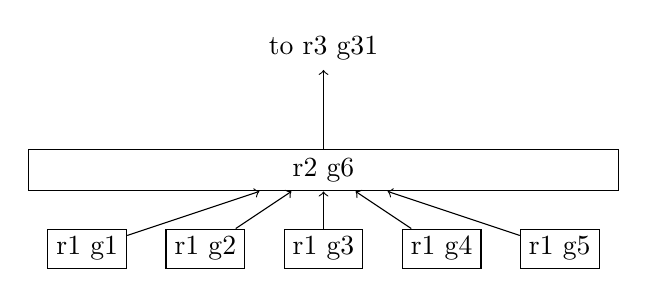
\begin{tikzpicture}[node distance=1cm and 1cm]
        % Bottom level blocks (5 participants)
        \foreach \x in {1,...,5} {
            \node[draw, rectangle, minimum width=1cm, minimum height=0.5cm] (P-\x) at (\x*1.5, 0) {};
            % Add "Rank X" text inside each block
            \node at (\x*1.5, 0) {r1 g\x};
        }

        % Single block for the game
        \node[draw, rectangle, minimum width=7.5cm, minimum height=0.5cm] (Game) at (4.5, 1) {r2 g6};

        % Connect participants to the game
        \foreach \x in {1,...,5}
            \draw[->] (P-\x) -- (Game);

        % Arrow pointing upwards from the top block with text "to r3"
        \draw[->] (Game.north) -- ++(0,1) node[above] {to r3 g31};
    \end{tikzpicture}
    \caption{Diagram illustrating the rank ladder. With minimum participant requirements of 5, 30 games are required to create a rank 3 game. Strong candidate would need only 2 wins to reach it.}
    \label{fig:game-connection}
\end{figure}


\end{document}
    The group can finalize only after $T_{i}$ has elapsed since the start state transition. Then a winner can be declared and his rank $P_r$ in the state trie incremented to $P_r=P_r+1$ only if group rank $R$ equals $P_r$ before finalization. This process can repeat and is illustrated in Fig. \ref*{fig:game-connection}.

    The staked assets were distributed to avoid a positive feedback loop between groups and participants. For example, nullifying these would incur the intrinsic cost of $X_{id}$.

    \paragraph{Dynamic Proof-of-Authority.} The state transfer is unidirectional from assets to rank and time-dependent. This makes every transition a differential equation cost:

    \begin{equation}
        \label{eq:time-weighted-proof-of-authority}
        \$P_r = \$(P_r-1) + X_{id}
    \end{equation}
    The rate of obtaining any rank $P_r$ is a unit step function dependent on time $t$:
    \begin{equation}
        \label{eq:time-weighted-proof-of-authority-1}
        P_r(t) = \lfloor \dfrac{t \cdot P_t \cdot P_c}{T_{min}} \rfloor
    \end{equation}

    \paragraph*{Frequency domain.} Eq.\ref{eq:time-weighted-proof-of-authority-1} highlights the dynamic nature of the protocol. Since it shows linear-time invariant property, the dynamic systems theory\cite{Lynn86} may be applied to analyze its stability and predict its future behavior.
    $1/T_{min}$ represents frequency, hence phase and frequency relationships between groups exist. Analysis my be done in s-domain using Laplace transforms. Different ${T_{min}}$ participants would result in a dynamic competence ladder that can produce specific quorums at specific times.

    \section{Sybil Attack Resistance}

    The protocol’s outcome represents an agent’s competence by storing his $R$ rank in the state trie. To ensure this representation isn’t manipulatable, we must analyze security concerns.

    From a game theory perspective, an adversary can be a group producing a winner with $R$ rank higher than any other group. However, the payment requirement in Eq. \ref{eq:group-fee} will be proportional to the number of participants, contrary to the stake requirement fair participants are expected to pay (Eq. \ref{eq:join-fee}).

    Principal components defining fees ensure any winner from any group is time and asset effort normalized.

    If $T_{min} = P_t$, then equation \ref{eq:group-fee} reduces to:

    \begin{equation}
        \label{eq:join-fee-2}
        X_i = P_c
    \end{equation}

    If one participant's rank $R$ transition requires a commitment from $N_{min}$ participants, such as a participation fee $X_i$, we can demonstrate that the proposed ranking ladder introduces a non-linear compounding friction for malicious actors attempting to manipulate the system. The strategy depends on the application of how the agents decide on the winner for such an adversary. If the process is deterministic, the expected cost is

    \begin{equation}\
        \label{eq:direct-sybil-cost}
        X_g \cdot N_{min}^R
    \end{equation}
    If an adversary can mix with fair non-sybil agents and the process is not fully deterministic, we can use the mathematical expectation for costs achieving specific rank via sybil attack described as
    \begin{equation}
        \mathbb{E}[\$R] = X_g \cdot \mathbb{E}[N_{\text{sybils}}(R)]
    \end{equation}

    Where $N_{sybils}(R)$ is the number of sybil accounts required to take quorum in a group and obtain rank $R$.
    \paragraph{Actor likeliness and group fragmentation.}
    From Eq. \ref{eq:direct-sybil-cost}, higher groups are more expensive to manipulate. However, breaking them into smaller ones may prevent communication complexity. This implies that due to group fragmentation, an attacker mixing sybil accounts with fair players must allocate accounts across groups for cost efficiency.

    Participants must assess the likelihood of a specific group being a sybil attack. If a group seems likely to be a sybil attack, participants must be able to opt out. This can be done by reviewing the past state history of participants, groups they are joining, and the social graph from vote allocation, using the dynamic systems methodology proposed in the previous section.

    While providing this visibility for participants may seem challenging, protocols like Continuous Voting Proposing Protocol (CVPP) \cite{cvpp} offer clear definitions for transparent systems. An automated system can analyze the state trie and provide a clear view.

    We can use additional verification mechanisms like proof of location \cite{sheng2024bftpolocbyzantinefortifiedtrigonometric} or proof of personhood \cite{WorldCoin2024} or quadratic voting systems proven helpful in blockchain governance \cite{Buterin20}\cite{Benhaim2024}.

    If all results are visible and easy to reason about, then for any protocol participant, confidence over a sybil attack increases as $R$ of the group increases. This leads to a higher likelihood of refusing to join such a group, resulting a sybil attack cost close to Eq. \ref{eq:direct-sybil-cost}:

    \begin{equation}
        \lim_{R \to \infty} \mathbb{E}[N_{\text{sybils}}(R)] = N_{\text{min}}
        \label{eq:limit-nmin}
    \end{equation} Where $N_{min}$ is the required number of peers to join the group. Eq. \ref{eq:direct-sybil-cost} estimates the cost of a sybil attack. For an agent relying on competence and winning each group fairly, the cost would be only
    \begin{equation}
        \$R = stake*R
    \end{equation}
    When making an arbitrary decision using $R$ as stake, this may involve taking privileged action with optimistic approval. The only condition to keep agent game-theoretically fair is that action impact must be lower than the cost of obtaining rank.
    \begin{equation}
        \$TVL <<  X_g \cdot N_{min}^R
    \end{equation}

    Total value locked must be lower than the cost for obtaining rank due to empirical studies needed to see how fast the required sybil count converges (Eq. \ref{eq:limit-nmin}) with different voting systems. This depends on the stochasticity and transparency of the process.

    \subsection{Quorum Resonances}
    \label{sec:time-constraint}

    As discussed earlier, any overt Sybil attack requires multiple groups to establish a sufficient ranking within the system. The intrinsic value of a tokenized competence rating is determined by financial effort, peer success, and time invested in improving one's position. An attacker needs $t_{attack}(R) = t_c \cdot R$ time to reach rank $R$. This duration allows protocol members to detect and respond to the attack.

    The Eq. \ref{eq:time-weighted-proof-of-authority-1} shows that system can be analyzed in time and frequency domains. This allows Sybil attacks analysis based on time, phase, and complex frequency domain analysis.

    Given the initial goal to facilitate protocol for subjective reasoning, it's unclear what a "Sybil attack" or a "different opinion" is. Assuming different opinions exist, and using the proposed s-domain methodology, competing groups can create a quorum resonance, where the opinion direction can oscillate. It takes the same $T_{min}$ for competing groups starting their election process at phase difference of $\pi$. This can be visualized in plot \Ref{fig:processes}.:

    \begin{figure}[ht]
        \centering
        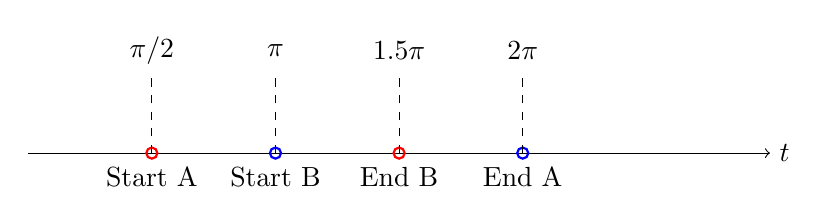
\begin{tikzpicture}
            % Define the x-axis
            \draw[->] (0,0) -- (3*3.14,0) node[right] {$t$};

            % Define the first process (point at Pi)
            \draw[blue, thick] (3.14,0) circle (2pt);
            \draw[blue, thick] (3.14*2,0) circle (2pt);
            \node[] at (3.14*0.5,1.3) {$\pi/2$};
            \node[] at (3.14,1.3) {$\pi$};
            \node[] at (3.14*1.5,1.3) {$1.5\pi$};
            \node[] at (3.14*2,1.3) {$2\pi$};

            % Define the second process (point at Pi/2)
            \draw[red, thick] (1.57,0) circle (2pt);
            \draw[red, thick] (1.57+3.14,0) circle (2pt);

            % Add labels for the timing diagram
            \node at (1.57,-0.3) {Start A};
            \node at (3.14,-0.3) {Start B};
            \node at (3.14*2,-0.3) {End A};
            \node at (1.57+3.14,-0.3) {End B};

            % Add dashed lines to indicate the timing
            \draw[dashed] (1.57,0) -- (1.57,1);
            \draw[dashed] (3.14,0) -- (3.14,1);
            \draw[dashed] (3.14*2,0) -- (3.14*2,1);
            \draw[dashed] (1.57+3.14,0) -- (1.57+3.14,1);
        \end{tikzpicture}
        \caption{Timing diagram showing two opposite opinion groups completing their election process at different times. The groups have the same $T_{min}$ with a phase difference of $\pi$.}
        \label{fig:processes}
    \end{figure}

    If many groups allocate their reasoning power in alliance, more complicated systems can be imagined. These can create local quorum resonances, analyzable in frequency domain, to predict future behavior \ref{fig:processes-sinusoidal}.

    \begin{figure}[ht]
        \centering
        \begin{tikzpicture}
            % Define the x-axis
            \draw[->] (0,0) -- (10,0) node[right] {$T_{min}$};

            % Define the y-axis
            \draw[->] (0,-2) -- (0,2) node[above] {Quorum power};

            % Define the first process (sine wave)
            \draw[domain=0:10,smooth,variable=\t,blue] plot ({\t},{sin(360*\t/10)});
            \node[blue] at (10,1) {Opinion 1};

            % Define the second process (sine wave shifted by half period)
            \draw[domain=0:10,smooth,variable=\t,red] plot ({\t},{sin(360*\t/10 + 180)});
            \node[red] at (10,-1) {Opinion 2};

            % Add labels for the half period shift
            \draw[dashed] (5,-2) -- (5,2);
            \node at (5,-2.5) {$\pi$};

            % Add labels for the full period
            \draw[dashed] (10,-2) -- (10,2);
            \node at (10,-2.5) {$2\pi$};

        \end{tikzpicture}
        \caption{Diagram showing two competing opinion groups over the same subject with the same $T_{min}$ but a $\pi$ phase difference. Sinusoidal waves illustrate their ability to strategically allocate their ranking on the time axis. In reality, the groups have different $T_{min}$ and could be more complex.
            \label{fig:processes-sinusoidal}}
    \end{figure}

    \subsection*{Utility of the allocated funds}
    The allocated funds can’t be directly used to reward winners and must be locked in representation of rank $R$. If used to reward winners, the system would be subject to manipulation by the highest bidder. This is a key feature of the protocol that ensures the ranking system isn’t manipulated by financial power.

    The financial asset can fund any underlying protocol utility for the discussion. If used with CVPP\cite{cvpp}, the funds can guarantee data availability of the discussion in a specific group, ensuring transparency in Sybil attack resistance. Protocols allowing on-chain payments for long-term data availability like Swarm \cite{swarm} ensure data availability by allowing operators to pull budget from the group's account.

    \section{Conclusion}

    This paper introduces a novel protocol for establishing a dynamic ranking ladder system in trustless environments. Our protocol enables autonomous identification while mitigating Sybil attacks by leveraging game-theoretic principles and dynamic systems theory. The time-based and cost-based mechanisms ensure high ranks require genuine effort and skill, and opposite opinions can co-exist.

    This protocol offers a foundation for building more robust and equitable decentralized governance systems. It improves blockchain consensus mechanisms, enhances DAO decision-making, and fosters healthier online communities.

    Further work is needed to analyze the protocol's behavior and effectiveness using dynamic system theory and explore its integration with existing decentralized platforms.

    \clearpage

    \bibliographystyle{ieeetr}
    \bibliography{../references.bib}

    \clearpage\end{CJK}
\end{document}
